% =============================================================================
% 5. MODELO DE NEGOCIO
% =============================================================================
\section{Modelo de negocio}
\label{sec:business-model}

\subsection{Contexto econ\'omico}

El mercado global de IA en radiolog\'ia se proyecta desde USD 0.76 mil millones en 2024 a USD 2.27 mil millones en 2030 (CAGR 24.5\%) \cite{marketsandmarkets2025}, con la FDA habiendo autorizado 1,451 dispositivos de IA, de los cuales el 76\% corresponden a radiolog\'ia \cite{fda2026aidevices}. Este crecimiento responde a una necesidad operativa concreta: los radi\'ologos en EE.UU. interpretan en promedio 49.4 ex\'amenes diarios, con el cuartil superior leyendo 30.6\% m\'as que en 2018 \cite{mcdonald2015workload}, evidenciando una carga laboral insostenible sin asistencia tecnol\'ogica.

\subsection{Impacto operativo documentado}

La evidencia cl\'inica respalda el impacto de la IA en radiolog\'ia (Tabla~\ref{tab:impact}):

\begin{table}[H]
\centering
\caption{Evidencia de impacto operativo de IA en CXR.}
\label{tab:impact}
\small
\begin{tabular}{lcc}
\toprule
\textbf{M\'etrica} & \textbf{Valor} & \textbf{Fuente} \\
\midrule
Reducci\'on tiempo lectura & 10--17.6\% & \cite{shin2023ai} \\
Aumento sensibilidad & +6.6 pp & \cite{ahn2022lunit} \\
Reducci\'on errores/caso & 0.38 $\to$ 0.27 & \cite{kapoor2025workflow} \\
ROI a 5 a\~nos & +451\% a +791\% & \cite{vanleeuwen2024roi} \\
Reducci\'on carga doble lectura & 44\% & \cite{lang2023masai} \\
\bottomrule
\end{tabular}
\end{table}

En particular, \cite{ahn2022lunit} demostraron en un estudio prospectivo con 6 radi\'ologos y 497 CXR que la asistencia de Lunit INSIGHT CXR aument\'o la sensibilidad de 0.715 a 0.781 sin incrementar el tiempo de lectura. \cite{vanleeuwen2024roi} cuantificaron un ROI de +451\% considerando ahorro de personal, que se incrementa a +791\% al incluir el tiempo liberado del radi\'ologo.

\subsection{Estrategias accionables}

\begin{enumerate}
    \item \textbf{Triaje autom\'atico en urgencias}: priorizaci\'on de casos con alta probabilidad de patolog\'ia para lectura humana inmediata. Sistemas como TRIA (CE Clase IIa) alcanzan AUROC = 0.911 en validaci\'on externa real.
    \item \textbf{Filtrado de estudios normales}: el 60--70\% de radiograf\'ias son normales; el modelo las identifica, liberando al radi\'ologo para casos patol\'ogicos. Esto genera un ahorro de $\sim$1 hora/d\'ia/radi\'ologo.
    \item \textbf{Screening masivo en zonas rurales}: pilotos en poblaciones tribales remotas han demostrado que la IA + CXR port\'atil identifica casos asintom\'aticos que el screening por s\'intomas pierde.
    \item \textbf{Control de calidad}: segunda lectura autom\'atica que reduce errores cl\'inicamente significativos de 0.38 a 0.27 por caso \cite{kapoor2025workflow}.
\end{enumerate}

\subsection{Limitaciones}

\begin{figure}[H]
    \centering
    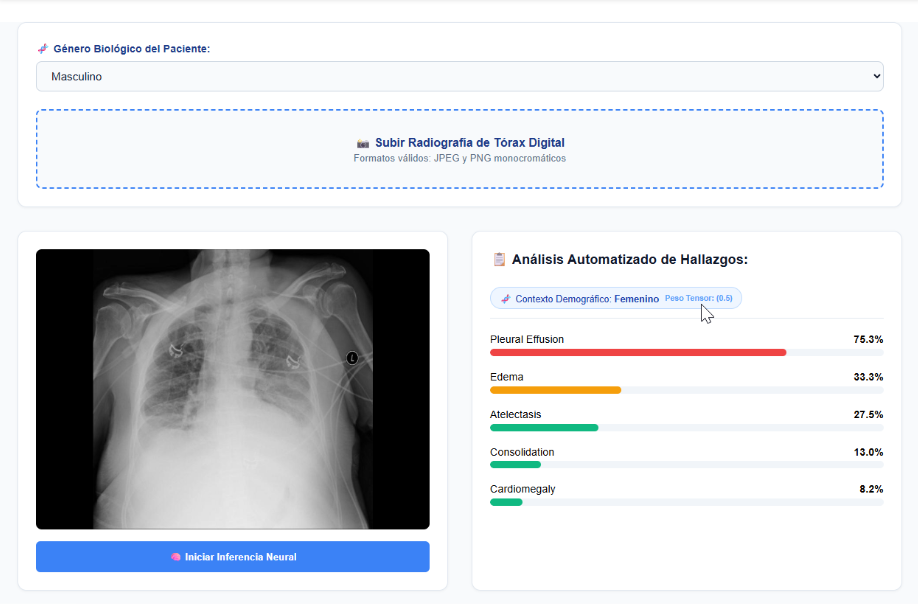
\includegraphics[width=\columnwidth]{figures/fullstack-plus-model-application.png}
    \caption{Aplicativo fullstack desplegado: frontend Angular + backend FastAPI con modelo ONNX integrado para inferencia en tiempo real ($\sim$20ms por radiograf\'ia).}
    \label{fig:fullstack-app}
\end{figure}

\begin{itemize}
    \item No es diagn\'ostico definitivo: es herramienta de screening y priorizaci\'on.
    \item Requiere supervisi\'on humana obligatoria (regulaci\'on m\'edica).
    \item El modelo presenta ca\'ida de 7.2\% en datos externos (requiere adaptaci\'on por hospital).
    \item Validaci\'on cl\'inica prospectiva necesaria antes del uso con pacientes reales.
\end{itemize}
